%-------------------------------------------------------------------------------
%	CAPITOLO 17
%-------------------------------------------------------------------------------

\chapter{Tre teste da capestro tutte e tre}
Il vecchio conte \index[Personaggi]{Foschini Camillo (conte)}Foschini era padrone ed abitava la casa \index[Luoghi]{Alberani (palazzo)}Alberani\footnote{\textbf{Palazzo Alberani}, La casa della famiglia del Dott. \index[Personaggi]{Alberani Anselmo}Anselmo Alberani, uno dei più ricchi proprietari terrieri di Alfonsine, in via Reale (dove oggi c'è la fabbrica di trasformazione “Contarini”). Era il padre di Alberto Alberani, che fu sindaco di Alfonsine.}. Una sera faceva la partita nella camera da pranzo, con amici, tra i quali \index[Personaggi]{Don Salvatori Ruggero}Don Ruggero. Era irrequieto, si contorceva sulla sedia, sembrava sugli spini. Accese un lume ad olio, disse agli amici: <<Vengo subito.>> e sparì. È da dire che il vecchio conte era un accanito papalino, mentre suo figlio \index[Personaggi]{Foschini Stefano}Stefano era liberale carbonaro\footnote{La Carboneria è stata una società segreta rivoluzionaria italiana, nata nell'allora Regno di Napoli durante i primi anni dell'Ottocento su valori patriottici e liberali.} acceso. \\
\indent In una camera superiore della casa erano a confabulare \index[Personaggi]{Farini Luigi Carlo}Luigi Carlo Farini\footnote{\textbf{Luigi Carlo Farini} (Russi, 22 ottobre 1812 – Quarto, 1 agosto 1866) è stato un medico, storico e politico italiano, per breve tempo Presidente del Consiglio dei ministri del Regno d'Italia tra il 1862 e il 1863.} il futuro dittatore e Ministro, \index[Personaggi]{Strocchi Girolamo}Momo Strocchi\footnote{\textbf{Strocchi Girolamo}, figlio di \index[Personaggi]{Strocchi Dionigi}Dionigi Strocchi che era stato un letterato, grecista e latinista italiano, amico di \index[Personaggi]{Monti Vincenzo}Vincenzo Monti. Nasce da Dionigi nel 1812. Da sempre cospiratore anche se mai vicino alle posizioni mazziniane estreme, è costretto ad esulare nel 1843. Rientrato a Faenza nel 1848 è capitano con il battaglione di volontari faentini che combatte a Vicenza e l'anno successivo viene arrestato dalle autorità pontificie. Nel 1850 è nominato colonnello della Guardia Nazionale. Con l'Unità d'Italia è più volte consigliere ed assessore comunale. Muore a Faenza nel 1885.} liberale faentino ed il conte \index[Personaggi]{Foschini Stefano}Stefano\footnote{Farini, Strocchi e Foschini erano tre rivoluzionari liberali che parteciparono al moto antipapalino di Romagna del 1843.}. Il vecchio conte padre si mise ad origliare dietro la porta i colloqui. Udito che ebbe che parlavano di politica, aprì la porta come un fulmine, col lume nella sinistra, la destra e l'indice teso si rivolse ai presenti indicandoli: <<Uno, due, tre, tre teste da capestro tutte tre\footnote{<<Tre teste da legare/impiccare>>}>>.\\
\indent Voltò le spalle, richiuse la porta e discese in fretta dagli amici, ridendo e dicendo: <<Credevo che facessero firmare cambiali a mio figlio... invece parlano di politica!>>\\
\indent Dopo il temporale era venuto il sereno nella faccia del vecchio conte, le cambiali erano uno sturbo\footnote{Scompiglio} forte... trasgredire ai suoi principi politici era cosa sopportabile!

 \begin{figure}[htb]
    \centering
    \vspace{-0.2cm}
    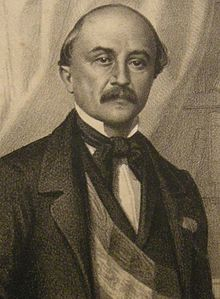
\includegraphics[width=0.8\textwidth]{farini}
    \caption[Luigi Carlo Farini]{\textbf{Luigi Carlo Farini}\\ Russi, 22 ottobre 1812 - Quarto, 1 agosto 1866\index[Personaggi]{Farini Luigi Carlo}\label{fig:farini}}
    \vspace{-0.4cm}
\end{figure}